\documentclass[journel,12pt,twocolumn]{article}
\usepackage{graphicx}
\usepackage[none]{hyphenat}
\usepackage{graphicx}
\usepackage{listings}
\usepackage[english]{babel}
\usepackage{graphicx}
\usepackage{caption} 
\usepackage{booktabs}
\usepackage{array}
\usepackage{amssymb} % for \because
\usepackage{amsmath}   % for having text in math mode
\usepackage{extarrows} % for Row operations arrows
\usepackage{listings}
\usepackage[utf8]{inputenc}
\lstset{
  frame=single,
  breaklines=true
}
\usepackage{hyperref}
  
%Following 2 lines were added to remove the blank page at the beginning
\usepackage{atbegshi}% http://ctan.org/pkg/atbegshi
\AtBeginDocument{\AtBeginShipoutNext{\AtBeginShipoutDiscard}}


%New macro definitions
\newcommand{\mydet}[1]{\ensuremath{\begin{vmatrix}#1\end{vmatrix}}}
\providecommand{\brak}[1]{\ensuremath{\left(#1\right)}}
\newcommand{\solution}{\noindent \textbf{Solution: }}
\newcommand{\myvec}[1]{\ensuremath{\begin{pmatrix}#1\end{pmatrix}}}
\providecommand{\norm}[1]{\left\lVert#1\right\rVert}
\providecommand{\abs}[1]{\left\vert#1\right\vert}
\let\vec\mathbf

\begin{document}
\begin{center}
\title{\textbf{Equation of Line}}
\date{\vspace{-5ex}} %Not to print date automatically
\maketitle
\end{center}
\section{11$^{th}$ Maths - Chapter 10}
\textbf{This is Problem-15 from Exercise 10.3}
\begin{enumerate}
\item The perpendicular from the origin to the line y=mx+c meets it at the point (-1,2) find value of $m$\text{ and } $c$.
\end{enumerate}
Solution:
\\
Given
\begin{align}
\vec{P}&=\myvec{-1\\2}\\
\vec{O}&=\myvec{0\\0}
\end{align}
The directional vector $\vec{OP}$ is 
\begin{align}
\myvec{\vec{O}-\vec{P}}^{\top}\vec{m}&=0\\
\implies\myvec{1&-2}\myvec{1\\m}&=0\\
\implies m&=\frac{1}{2}
\end{align}
From the line equation 
\begin{align}
\myvec{\frac{1}{2}&1}\myvec{\vec{x}-\vec{P}}&=0\\
\implies\myvec{\frac{1}{2}&1}\vec{x}&=\frac{5}{2}\\
\implies c&=\frac{5}{2}
\end{align}
\begin{figure}[!h]
\centering
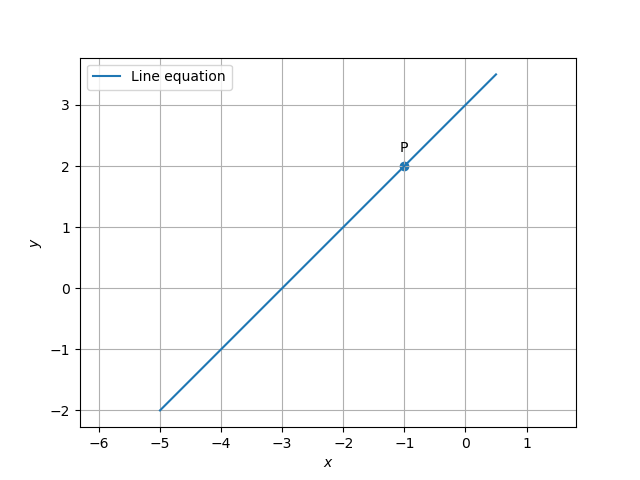
\includegraphics[width=\columnwidth]{fig.png}
\caption{}
  \label{fig:Figure}
\end{figure}
\end{document}